\documentclass[10pt,a4paper,twocolumn]{article}

\usepackage[top=1cm,bottom=2cm,left=2cm,right=2cm]{geometry}
\usepackage{graphicx}
\usepackage[backend=bibtex]{biblatex}
\usepackage{hyperref}
\usepackage{amsmath}
\usepackage{xcolor}
\usepackage{listings}
\bibliography{report.bib}
\author{Christoffer Jansson \and Alan Khudur \and Dmitrij Lioubartsev \and Michal Staniaszek \and Yavor Trasiev}
\title{DD2425 Robotics and Autonomous Systems Final Report}

\begin{document}
\maketitle
\begin{abstract}
  In this report we describe our hardware and software solutions for the house
  service robot task set in the DD2425 Robotics and Autonomous Systems course.
  The task required the construction of a robot from a limited set of materials,
  and the implementation of a software system using the Robot Operating System
  (ROS)\cite{rosorg} framework. We implemented a control system for motion in
  the maze, including wall following, a vision system to make use of the
  Primesense RGB-D camera, and additional systems for mapping.
\end{abstract}
\section{Task Specification}
The website for the course specifies the task as follows:
\begin{quote}
  \emph{Your robot is the new service robot is someone's house. The new owner has just
  turned on the robot and given it a few minutes to have a look around in the
  new environment. Your robot should take this chance to learn as much as
  possible about the environment so that it can be as good as possible in future
  tasks. It should learn to find its way and it should detect and remember where
  certain objects are.}
\end{quote}
This specification is a description of a real world task that might be performed
by a robot. Since we had only two months to implement the system, the actual
task that had to be performed was somewhat simplified. The ``house'' was
replaced by a maze made of straight pieces of wood, with all of the walls having
either a horizontal or vertical orientation --- there are no diagonal walls. The
robot should detect and remember the location of are various brightly coloured
shapes, seen in Figure~\ref{fig:shapes}.

The task can be broken into two phases, each of which has a distinct purpose. In
the first phase, the robot must explore the environment and learn where objects
are. In the second phase, which is not described explicitly in the
specification, the robot should return to the previously discovered object
locations and ``fetch'' the objects.

Although these tasks would be trivial for any human, for a robot to do them
autonomously is a very demanding task, even in a restricted environment such as
the one we will be operating in. To complete the first phase, we must be able to
move the robot, which requires the implementation of controllers which allow the
robot to move based on demands on angular and linear velocity. A wall following
system is also required, to use the structure of the environment to explore it.
This requires the use of sensors to detect walls to the side and in front of the
robot to prevent collisions, and detect when it is possible for the robot to
turn. A vision system which can detect objects and correctly identify them is
also needed. A map must also be constructed and stored so that the position of
objects can be remembered for use in the second phase. During the second phase,
some sort of path planning is required to move efficiently between the different
objects. The ability to localise within the created map is also necessary in
order for the robot to know the position of objects and walls relative to its
own location. In addition, a way of navigating between specific locations in the
map is required.

To complete the full task, we had to design and build a robot, and write
software for all of these subsystems. The subsequent sections describe our
approach to each problem and how we solved it, including some of the ideas that
we did not use, and the reasons for that, as well as some analysis of the
performance of each of the subsystems.


\section{Hardware}
We decided early in the project to build the robot onto a circular platform, so
that no part exceeds its radius. This was done in order to have a failsafe
mechanism in which the robot could rotate around the z-axis without much
problems if it would get stuck in corners and move on. Underneath the circular
platform the robot had its two motors with wheel, two caster wheels, six IR
sensors and the battery mounted. On top of the platform, the Intel NUC, Arduino
board and the Primesense camera were mounted. See Figure~\ref{fig:roboview}. 

As nice as it is to have a circular body that does not get geometrically stuck,
there is a lot of bulk to it, which is definitely felt in the tighter parts of
the maze. One could be forgiven to think it is better to solve this problem by
code instead of using the physical shape, and that’s probably true. However we
wanted to implement the solution as quickly and simply as possible. Also, our
idea for having symmetry meant having two support caster wheels. The problem
with having four support points is having them all aligned perfectly. This
warranted adjustable wheel carriers which had to either be a simple L-shape or
would have needed intricate holes to facilitate adjustment. We went with the
former, which resulted in them constantly bending up and since the caster wheels
have a significant offset this meant we couldn't steer. We fixed this issue by
adding an additional bracket.
\begin{figure}
  \centering
  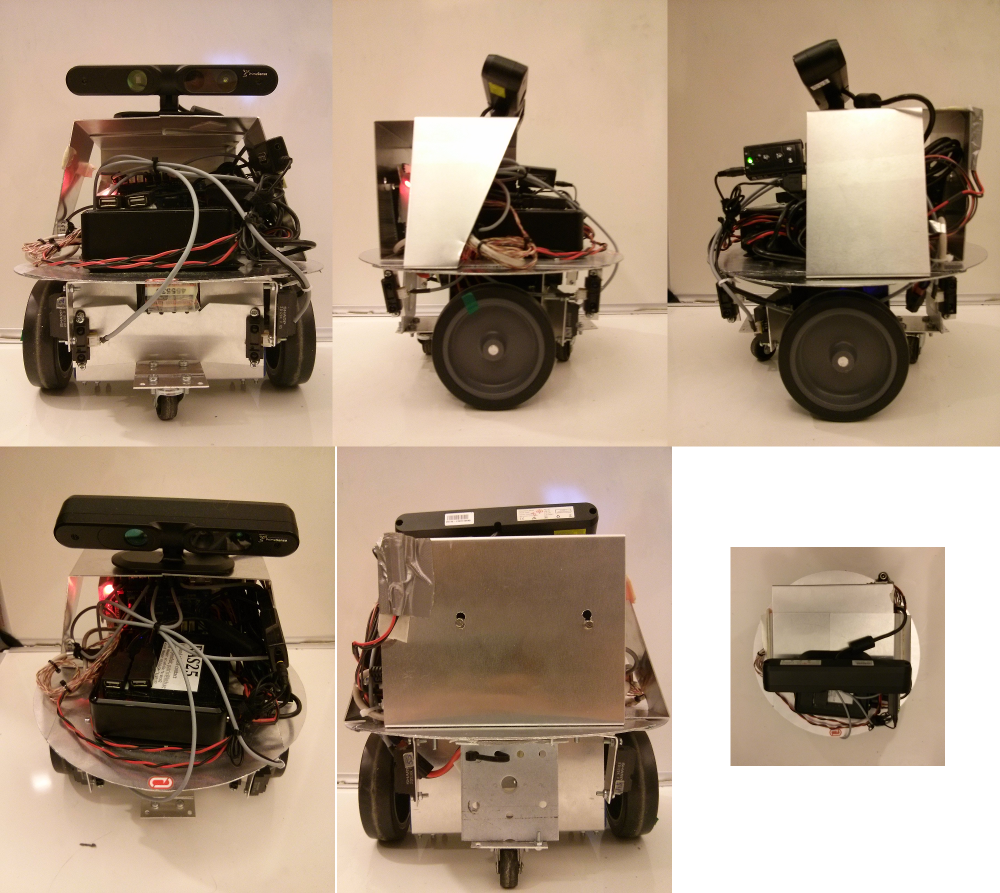
\includegraphics[width=\linewidth]{images/robo_views.png}
  \caption{Views of the robot from different angles.}
  \label{fig:roboview}
\end{figure}
\subsection{IR Sensors}
The robot used infrared sensors in order to detect obstructions in the
environment. For this particular project, the obstructions were walls in the
maze which the robot would traverse in. Six sensors were used - two long range
sensors of type Sharp GP2D120 and four short range sensors of type Sharp GP2D12.
The long range sensors were specified for a range of 10-80 cm while the short
range sensors for a range of 4-30 cm. The sensors were positioned in such way
that two short range sensors were mounted on the left respectively on the right
side and the remaining two long distance sensors on the front side of the robot.
The purpose of this layout was to use the side sensors to detect, follow and
avoid collisions with the walls in the maze while the front sensors would be
able to detect any obstructions such as object or walls in front of the robot.
The front sensors were positioned in an angle towards each other so that any
thin obstructions which could lie in between these two sensors could be detected
(see top left-most image in Figure~\ref{fig:roboview}).

The output of the sensors were numbers ranging from 0 to 550 for the long range
sensors and 100-550 for the short range sensors. Each number corresponded to the
distance from the sensor where a higher number indicated that an object were
closer to the sensor. The correlation between the raw data and the distance was
exponential and the raw data contained a lot of noise, making readings of the
raw data in real time neigh impossible.  In order to solve this problem the
sensors had to be calibrated. This was done using a movable wall which was
positioned orthogonally to each sensor. For each distance (between 4-30 cm for
the short range sensors and 10-80 cm for the long range sensors) data was
recorded using rosbag for a couple of seconds. The wall, starting from the
closest position each sensor could register, was moved 2 cm backwards in between
each reading in order to minimize the amount of data points as it would be too
tedious to process later on.  When the collection of the data was done, each
rosbag was extracted of its data and put in a separate text file. The text files
were read to Microsoft Excel in where all data for each distance and sensor was
extracted. This extracted data was later read to MathWorks MATLAB where the mean
value for all collected data for each distance and sensor was calculated (we
discussed if we were to use the mean or the median, but decided on the mean for
now since the difference was minimal). For each sensor, each distance point we
used could now be plotted as a function of the calculated mean values and fitted
with MATLAB’s built-in tool cftool using a polynomial curve which later, after a
couple of recalibrations, was changed to an exponential curve due to problems of
unexpected curvature between several calculated points. All exponential curves
which were fitted were of second degree in form of: 
\begin{equation}
  \label{eqn:eq1}
  f(x) = ae^{bx}+ce^{dx}    
\end{equation}


MATLAB was kind enough to calculate and return the values of the constants $a,
b, c$ and $d$. This was later added to a C++ node in which raw output data from
each of the sensors were read, added as the $x$-value in equation~\ref{eqn:eq1}
and published all in real-time for later use in the wallfollowing and
exploration controllers.

\begin{figure}
  \centering
  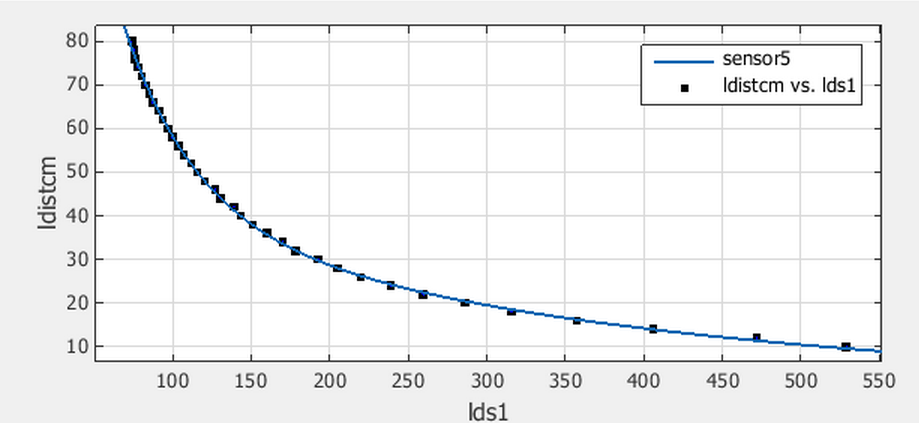
\includegraphics[width=\linewidth]{images/sensorcalib.png}  
  \caption{Distance in cm as a function of the raw sensor data given by a long range sensor.}
  \label{fig:sensorcalib}
\end{figure}

Unfortunately, the sensors given to us were of low quality and had a tendency to
switch the returned values for every distance every day, forcing to be
recalibrated. At first, this issue was battled and several recalibrations were
made, but later on this issue was neglected and instead adapted to in the
wallfollower. Another problem was that the sensors had problems outputting
correct distances close to the limit of the sensor ranges which was solved by
putting the sensors closer to the center of the circle (see Section~\ref{sec:wall}).

\section{Controllers}
Controllers are needed to regulate all the motion-related systems not only on
the low level (e.g. direct motor control) but on a higher level as well --- for
example, a wallflower controller that controls the input of the motor controller
in order to align the robot to the wall. This is not always the optimal
solution, since each controller introduces some lag and imprecision, so the
final result may be of poor quality no matter the amount of controller tuning.
This is why some of the controllers used were direct controllers, i.e. they had
a direct control of the motors. Unfortunately, this means that there was no way
to have a neat single motor controller that runs in the background and awaits
commands, but rather a bloated node with two distinct controllers in it --- one
for roaming and wallfoling and one for precision turning.

\subsection{Motor Controller Node}
The structure of the node is such, that at any given moment, the robot is either
static, or in one of two modes: free-roaming mode or precision turning. It
consists of two controllers, each of which controls one of the motors.
Obviously, the difference in the velocities of each wheels defines the dynamics
of the robot, so this is used through a motion model to either control the rate
of turning of the whole robot while keeping a constant linear velocity, or the
total distance each wheel travels to achieve a rotation of the robot with zero
linear velocity. This is node that accepts a Twist message which defines the
linear speed and angular velocity of the robot in free-roam mode, and a turn
value, which unless set to 0, defines a precision turning reference in degrees.
After each transition of the states the memory of the controller is
reinitialized to make sure there is no windup. That said, there was a certain
set of cases where there windup occurred frequently which meant we needed to ad
anti-windup measures and take that into account during the tuning. The node also
communicates with the Master node (Explorer) by conveying a message for whether
it has finished turning or not.

\begin{figure}
  \centering
  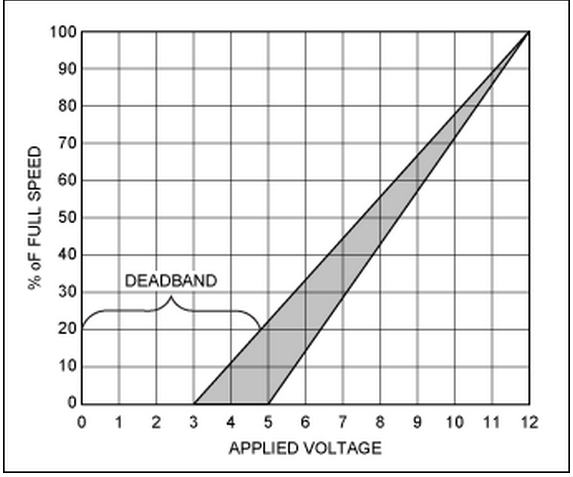
\includegraphics[width=\linewidth]{images/deadband.png}
  \caption{Nonlinearity of DC motors: hysteresis and deadzone.}
  \label{fig:deadband}
\end{figure}
\subsection{Tuning}
Each mode was tuned separately, because of the nonlinearity of the motors. As
seen in Figure~\ref{fig:deadband}, the hysteresis and deadband of the motors,
accentuated by the lossy non-linear gearbox makes control of the left and right
motors highly dependent on each other. Another complication was the fact that
the reference for the roaming mode for each motor was the linear velocity of the
wheel, and for the precision turning mode the reference was the distance
traveled. All this meant that two set of tuning parameters had to be derived,
taking into account the if the direction of the wheels was the same or opposite.
A nearly perfect control was achieved by using a bias on the control output
which was carefully selected by the characteristic of each motor in each
direction of rotation. Although there are hundreds of pre-determined methods for
controller tuning, most of them require a highly sophisticated model which could
not be justified by our team --- it would have taken more than two weeks to
complete, while the ``by eye'' tuning approach which relies on experience and
understanding of the control algorithms and motor characteristics took much
less. Unfortunately there were more problems: 
\begin{enumerate}
\item the motors deteriorated to the point where their output speed was up to
  30\% lower for the same voltage. This process was continuous and we had to
  tune at least 3 times to compensate for it.
\item The battery position really affected the weight distribution --- because it was
not completely fixed the weight would shift from the front to the rear caster
wheels, causing massive problems with calibration due to uneven caster wheel
carriers.
\end{enumerate}

\subsection{Wall Follower}
The type of controllers we used we mainly PID (more
\href{http://lmgtfy.com/?q=PID+tutorial}{here}), however the wall following
worked just fine with only a P controller due to the inherent inertness of the
system and the fact that it controls the reference input of the main motor
controller node. The controller uses the difference between the front and rear
sensors on a particular side to control a reference value for the main motor
controller.

\section{Wall Following and Exploration}
\subsection{Wall Follower}
\label{sec:wall}
Figure~\ref{fig:maze} shows the test maze that we had to work with. The robot
was designed to be round to avoid situations where it got stuck in corners or
unable to turn in any position. This design although well intended meant that
the robot had to be quite wide which leaves little room for error when turning.
The robot is 28 centimeters wide at any point and the maze is approximately 40
cm wide meaning that the robot have 5-6 cm on each side when going through a
corridor in the maze. This means that the wall following have to be quite
accurate and not stray too far from the straight path in the middle. Hitting or
bouncing into the walls will throw off the odometry of the robot and result and
adversely affect the mapping. The original wallfollower node was written to
subscribe to raw data from the arduino sensors for wall following and encoders
for determining when to stop turning. The wall following part was done following
the left wall with a simple P controller and was simply based on following the
wall and when the left wall ends try to turn left. To determine when to turn a
“state” machine was written using a integer. This solution was working poorly so
a new version wallfollower2 was written. Wallfollower2 used a byte to store
information about which sensor had contact with the wall resulting in a value
between 0 and 63. This value was then used to assign a function pointer
reference from an array of function pointers to a function pointer that was
called each cycle. This had the disadvantage that you had to make 64 functions
to get all possible states to work which seemed ineffective so another program
was written named simple explorer.

\begin{figure}
  \centering
  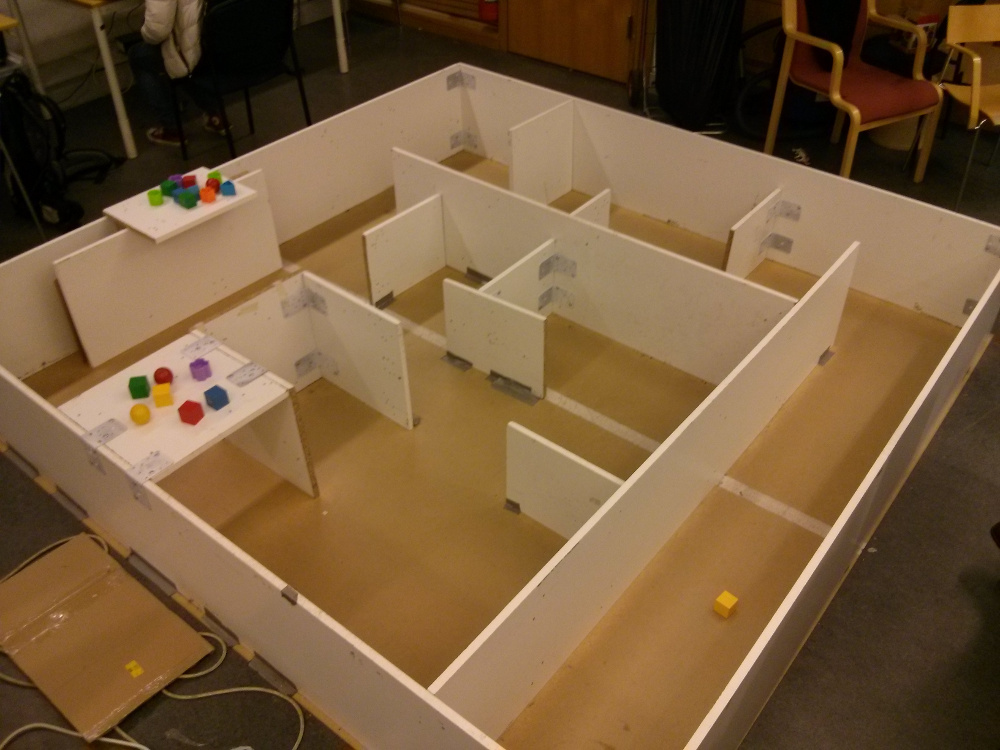
\includegraphics[width=\linewidth]{images/maze.jpg}
  \caption{The maze}
  \label{fig:maze}
\end{figure}
\subsection{Explorer}
The simple explorer uses the same principle of storing sensor data in a byte but
had a separate integer that stored the state. This reduced the  number of
necessary state functions from 63 to 5. These states are if you dont have an
contact on the left side or the right side go forward. If sensor reading comes
from the front facing sensors turn 90 degrees to the left or right if there is
an obstacle registered by the left facing sensors. If there is contact on both
left facing sensors follow the left wall and if thats not the case try following
the right wall if the right facing sensors have contact. This however meant that
it was no longer a real left side wall follower so a complex explorer was
written to solve that situation. The complex explorer adds three states that
make sure that the robot always follows the wall on the left side. The first
state is if there is nothing on the left side sensors turn 90 degrees to the
left. After that using the left facing sensors to scan for a wall to follow or
if an edge of a wall is registred turns 90 degrees left and then drives forward.
The final state that was added was to turn 180 degrees if walls are registered
by all front sensors. This should result in a robot capable of traveling through
any maze however there were issues. The most severe issue was false sensor
readings which was solved by gathering a couple of sensor bytes after a change
has been made before changing state. Another limitation was the placing of the
front forward facing sensors which was placed 7.5 centimeters from the roll axis
of the robot. This means that the robot can only discover walls in front of it
if it was within a 15 centimeter from around the roll axis with a 28 centimeter
wide robot meaning that the robot had a blind spot of 4 centimeters on either
side facing forward. This was solved by stopping quite far from the wall for
turning making sure that the robot could follow the entire test maze to the end
in one go.

\section{Vision}
\begin{figure}
  \centering
  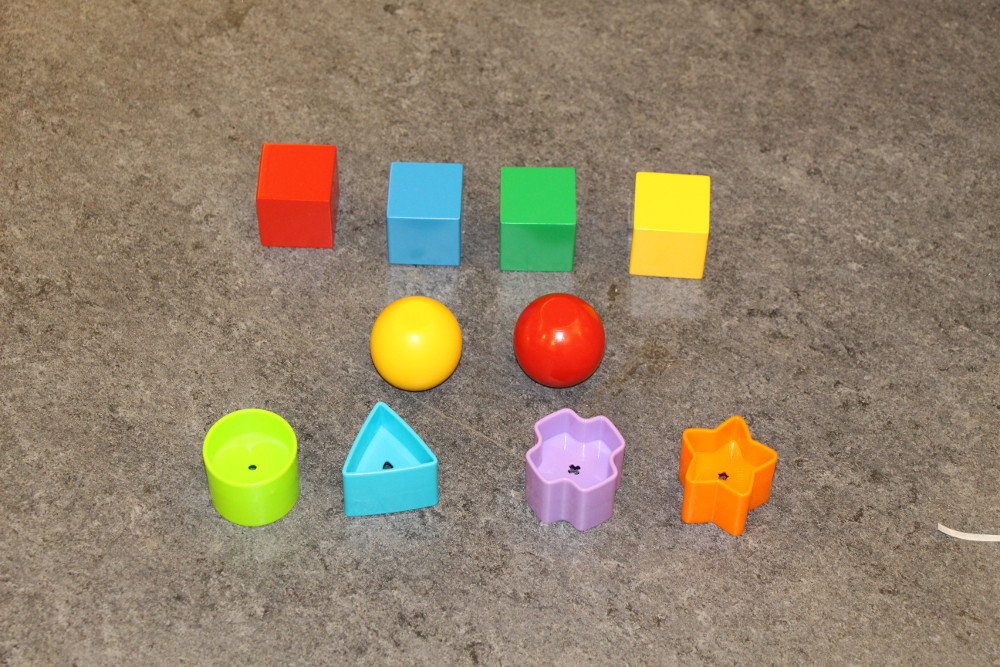
\includegraphics[width=\linewidth]{images/objects.jpg}
  \caption{Objects to be detected within the maze.}
  \label{fig:shapes}
\end{figure}
\subsection{Observations About Objects}
The object set can be seen in Figure~\ref{fig:shapes}. Each object only has one
color, and no texture features. There are objects of the same color but
different shapes and objects of the same shape but different colors. Because of
the lack of texture, feature-based detection\cite{feature} will not work very
well. However, because all objects are all mono-colored, some sort of detection
based on color is appropriate. Having only color detection is not enough though,
as objects with the same color need to be differentiated through shape. This can
be done with either looking at contours or utilizing the depth part of the
Primesense camera and looking at the object shape. We chose the shape method.

\subsection{Color Detection}
The objects can be separated into 6 different colors: blue, green, red, yellow,
orange and purple. The green objects and the blue objects are not exactly the
same color but they are similar enough to be grouped together.

For the color detection the RGB sensor of the Primesense camera was used. ”RGB
sensor” is a buzzword and it is more commonly known as simply “camera”. The
camera outputs an image stream. For each frame, we get an image encoded as an
RGB image. RGB stands for “Red Green Blue” and is the most common color
representation model. An image consists of many pixels. Each pixel uses three
values (usually between 0 and 255) to represent the amount of each color. For
example, (0,0,0) is black and (255,255,255) is white. Each combination of RGB
values yields a unique color, so this representation allows for 2563 different
colors. However, obviously colors with very similar values look very similar.
Changing just a few points in each value will barely be detectable by the human
eye. So while we can say that each object consists of only one color, that is
technically not true. Things like dirt, shadows and background/environment light
will change the object’s pixels’ values.

Because of this, we need to define a range of pixel values which represent each
color. In other words, each color will have a model. Then during detection, each
pixel will be compared to the model to get some number on how similar a pixel is
to the color. This is done for every pixel in the image in each frame. Then,
using a threshold, a threshold image is created. Basically, every pixel “similar
enough” is set to 1, and otherwise 0. Then we check if there is a big blob
somewhere, and if so, we say that we found an object of this certain color. We
used our own algorithms combined with OpenCV algorithms to build the color
detection system.

\subsection{Model Training}
The simplest color model would be to just put some threshold values directly on
the RGB values of each pixel. That has certain issues, as it is hard to know
exactly where the different thresholds somewhere, and if so, we say that we
found an object of this certain color. We used our own algorithms combined with
OpenCV algorithms to build the color detection system.

Model training The simplest color model would be to just put some threshold
values directly on the RGB values of each pixel. That has certain issues, as it
is hard to know exactly where the different thresholds should be. A thing to
note about the RGB encoding is that it contains data about light intensity. If
the ratio between the three values stays the same, but the values change, the
color stays the same, but just changes illumination (gets lighter/darker). To
make the model less affected by illumination, instead of using RGB
representation we transform all pixels to the $rg$-chromaticity
representation~\cite{rgchrom}. In short, given a pixel’s $R$, $G$ and $B$ values, we
calculate $r$ and $g$ as

\begin{align}
  r &= \frac{R}{R+G+B}\\
  g &= \frac{G}{R+G+B}
\end{align}

and use that as the representation in each pixel. This also simplifies the model
as it is only 2-dimensional now.

We also tried the representation used in~\cite{balkenius2007finding}. It did
however not yield better results, and was just generally slower, so we stuck to
just using rg-chromaticity.

For the model, we used a two-dimensional multivariate Gaussian to represent each
color. A two-dimensional Gaussian has in total 6 parameters: the means of each
colours (a 2-dimensional vector $\mu$) and the $2\times 2$ covariance matrix $\Sigma$
which represents standard deviation and co-variation. Using training data, we
calculated these parameters for each color using the formulas given
in~\cite{smean}. To summarize: $\mu$ is the mean vector, $x$ is the vector of all the
training pixels, and N is the number of training pixels. One could say that $x$ is
technically a $2\times N$ matrix.

\begin{align}
  \mu_i&=\frac{1}{N}\sum_{j=1}^Nx_{ij}\\
  \Sigma_{jk}&=\frac{1}{N-1}\sum_{i=1}^N(x_{ij}-\mu_j)(x_{ik}-\mu_k)
\end{align}

For the training data, we wrote a quick program with which we could take images
with the Primesense camera. At first we used our cell phone cameras but the
model was more accurate when we used the Primesense. The images were taken in
the test maze to get the training data to be as similar to the actual data as
possible. The objects were then extracted from the images and put on black
backgrounds using Photoshop. Photoshop’s quick selection tool made it very easy
to select the objects, and it took around 30 seconds per training image. The
process is shown in Figure~\ref{fig:purpim}. It took more time to save the new
images than actually select and extract the objects. Before using Photoshop, we
tried doing the extraction automatically by taking pictures of the objects on a
white background and using thresholding to extract the object from the image.
The extraction was quite fast, but often resulted in parts of the background
being included in the resulting image, which was negatively affecting the
training data. We decided that accuracy was more important than speed in this
case, and instead did the extraction manually.
\begin{figure}
  \centering
  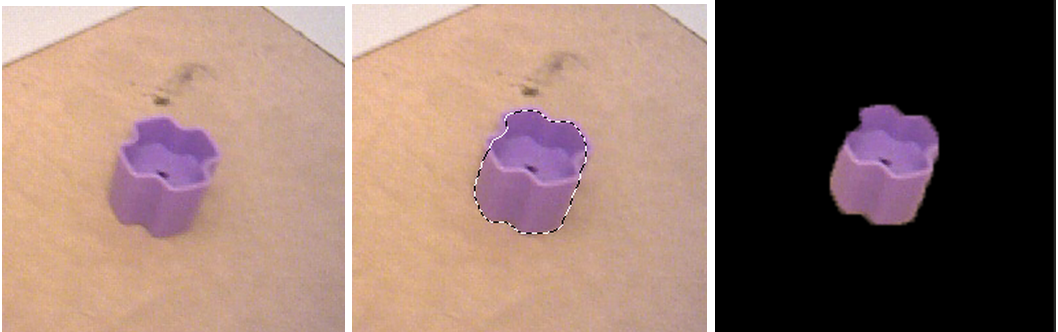
\includegraphics[width=\linewidth]{images/purpim.png}
  \caption{Training image, object selected (with 1 click), and then pasted onto a black background.}
  \label{fig:purpim}
\end{figure}
We used approximately 40 training images for each color. We wrote a program
which calculated the $\mu$ and $\Sigma$ from all images in a given directory. It
assumed that every non-black pixel was from the object, and then just used the
above formulas for the calculations. Because this is ran once, before we even
run the robot, this does not need to be efficient. This way we had a fairly good
framework for getting training data, and we could easily add new training images
or remove existing images.
\subsection{Detection}
When the robot is moving around in the maze, we get an image for each frame. We
first convert it to rg-chromaticity representation, and then using OpenCV blur
it a bit to lower the impact of noise. Then we calculate the similarity of each
pixel to the model (this is done once for each color). For this we simply insert
the pixel values into the Multivariate Gaussian formula
\begin{align}
  &pixel=\frac{1}{\sqrt{(2\pi)^2|\Sigma|}}\exp\left(-\frac{1}{2}(x-\mu)^T(x-\mu)\right)\\
  &  =\frac{1}{\sqrt{(2\pi)^2|\Sigma|}}\exp\left(-0.5(r_n^2\Sigma_{11}^{-1}+2r_ng_n\Sigma_{12}^{-1}+g_n^2\Sigma_{22}^{-1})\right)
\end{align}
Where $r_n= (r-\mu_r)$ and $r_g= (r-\mu_g)$. $|\Sigma|$ is the determinant of
$\Sigma$, and $\Sigma^{-1}$ is the inverse of $\Sigma$. Also note that
$\Sigma_{12}= \Sigma_{21}$ is always true. This is not very efficient
calculations to make for every pixel. Some simple optimizations can be made by
moving -0.5 into the big parenthesis. Because $\Sigma$ and $\mu$ never change
between runs (they are from the model), things like $\Sigma^{-1}$ and $|\Sigma|$
can be calculated only once upon start. In fact, the whole big thing left of the
exp can be pre-calculated. To make it even faster we calculate the natural
logarithm of the expression as well. Then we get

\begin{equation}
  pixel=c\cdot(r_nr_np_1+r_ng_np_2+g_ng_np_3)
\end{equation}
Where the $p_i$ is some pre-calculated variable. This means, that for this part
we only use 7 multiplications and 2 additions.

The next step in the algorithm is to make the threshold image. The threshold was
set without any training by trial-and-error. Because we calculated the logarithm
of the pixel value, we have to set the threshold to the logarithm of the
threshold. This is done once during startup so it is ok. The issue with doing
the threshold method is that we lose the similarity data. The strong part with
the gaussian model we use is that you get some sort of probability for each
pixel being that certain color. This information is lost with the thresholding.
We experimented with some ways of utilizing this data, but never got anything
successful working. With the thresholding, we could utilize the OpenCV algorithm
findContours.

findContours does what the name implies. It finds the contours in a binary
image. We then take a simple approach and simply check the size of the biggest
contour. If it is larger than a certain threshold, we say that the image
contains this particular color.

Note that everything above from blurring, is done once for each color every
frame. So we can detect multiple different colours in the same image.

\begin{figure}
  \centering
  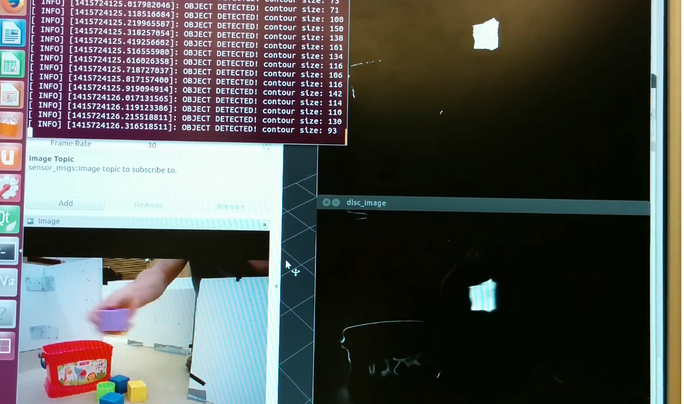
\includegraphics[width=\linewidth]{images/purpdetect.png}
  \caption{Purple color detection. Bottom left is the full RGB image. The bottom
    right is the image with the pixel values calculated from the model (brighter
    means more likely to be purple). Top right is the thresholded image. Top
    left is the console writing each frame if the color is detected or not.}
  \label{fig:purpledetect}
\end{figure}
\subsection{Shape Detection}
We made a key observation about the object dataset: objects of the same color
are either a cube or non-cube. This means, that if we could distinguish between
a cube and non-cube we could distinguish between all objects. So we needed the
shape detection to look for cubes. Another observation we made was that the cube
is the only shape which has a plane which is parallel to the floor. The circle
has one but it is significantly smaller. This crafted the ridiculously simple
idea, that we could just look for planes parallel to the floor in the
pointcloud. A pointcloud is the one of the outputs from the Primesense. It gives
a set of points with $x,y,z$ coordinates, essentially giving us a 3D image. Each
point also contained color information but we did not use it. We used the
library PCL~\cite{pclorg} to work with pointclouds.

The first step of the algorithm is to extract the floor. This is done with the
RANSAC algorithm which is provided by PCL. It extracts the dominant plane in a
pointcloud, which often is the floor, however when the robot drives close to a
wall it becomes the wall. It also gives the plane’s coefficients (on the form of
$ax+by+cz+d=0$). We identified the typical coefficients when the dominant plane
is a floor, and put in a check, so that we do not try and find cubes when the
dominant plane was a wall. We also tried a version where we extracted multiple
planes, but that did not work better.

Using the extracted plane’s coefficients and the pointcloud with the floor
removed, we ran the PCL algorithm NormalEstimation. This looks at each point,
takes its closest neighbors, assumes they are a plane, and calculates that
plane’s normal. This was quite slow on a large pointcloud so we downsampled the
pointcloud first (another PCL algorithm). In practice, this meant that all
pixels on the top side of a cube (except those close to the edge) would have
normals pointing straight up - same as the floor’s normal! Due to the
environment being so restricted, cubes are the only shapes that would get
normals pointing straight up, so we could just count the amount of normal
vectors pointing up, and if they were many enough we said there was a cube in
the image.

To check if a vector pointed upwards, we used the dot product between the floor
normal and the vector to get the angle between them. If the angle was low enough
(say, 5 degrees), the vector is said to be parallel with the floor.
\subsection{Vision Master}
Using the data from the color and the shape detection, we could identify which
object was in the image, if there was one. The color was used primarily to find
the object, and then the cube data (just a boolean) would be used to distinguish
which object it was of that color (if needed). This was done in the vision
master part of the program. If a certain object was seen for a certain amount of
frames in a short time, that object counts as found. Each object can only be
found once, as the vision did not keep track of where a certain object was
found.

To tell the mapping where the object was found, we used the depth data from the
Primesense, the Primesense Field of View values, the contour centers from the
color detection and the height the camera was positioned at (approx. 27 cm), we
could calculate the offsets in different axises where exactly the object was
positioned relative to the robot’s position.

This detection works fine (in theory!) if there is only one object in view. This
will not always work properly with more than one object in view. To fix that was
not our highest priority. But we did try a variation where we utilized the
position of where the object was found, and only looked for a cube in that
particular area. This could then be done for each color found, essentially
meaning that we could detect multiple different objects in the same view. Since
the color detection only took out the biggest contour, we still could not detect
both if there were two objects of the same colour in the same view. That is such
a rare case so we never bothered fixing it.

\subsection{Did it work?}
Well, kind of. Sometimes it worked great and other times not.

\subsubsection{Color}
The color worked really well for purple, blue and green. Especially purple. I
would be surprised if any other group was as good as us on the purple cross. See
Figure~\ref{fig:longpurple}. From over 1 meter distance, while the robot was
moving, it sees the purple cross while it is very badly illuminated. Blue and
green are not as insane but are quite good.
\begin{figure}
  \centering
  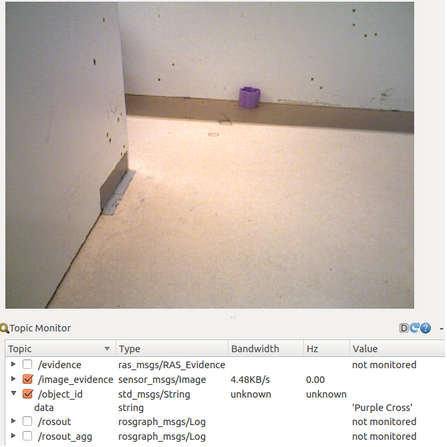
\includegraphics[width=\linewidth]{images/longpurple.png}
  \caption{Purple object detected, from the evidence viewer.}
  \label{fig:longpurple}
\end{figure}

The color yellow was not detected very well. We never adjusted the parameters
very well. But we were afraid to play with them too much as the floor was of a
similar color. Out in bright spots, yellow was detected decently.

Red was always detected fairly well. The problem was that red and orange were
extremely similar. We did not expect that. Red objects would often be
misclassified as the orange star, and vice versa. By the time we found this out
it was too late to do anything about it. Well, we tried taking training pictures
more carefully, but that made the models even more similar.

\subsubsection{Shape}
We did not spend nearly as much time on shape detection as on color detection,
and it shows. In theory, even though the idea is very simple, it should work.
And it did work in our initial tests. We could actually detect all 10 objects.
The thing is, that the robot was standing still. And the objects were on the
middle of an open floor.

When driving in the maze, there is more noise, and the objects typically stood
next to walls. Especially them standing close to walls really messed up the cube
detection. In attempt to fix this, we tried things like removing several
dominant planes (already mentioned) and looking for parallel vectors only in the
approximate area where the color detection found the object (also mentioned). To
try and reduce noise was actually the main motivation to try those things.
Unfortunately nothing of this worked, and then we were out of time.

\subsubsection{Contest}
Well, we never bothered adjusting the color detection to the vastly different
light conditions in the Ljusg{\aa}rden compared to the lab. Because of that, nothing
in the detection worked properly and we misclassified a lot of objects. Of
course, the purple cross was still detected correctly (when we tested in the
break).

\section{Mapping}
In order to perform the task required in the second phase more efficiently, we
need a map in which the location and type of object is stored, as well as the
locations of walls and other potential obstacles. To make the map we use only
the IR sensors. Using the Primesense as well might have given us more data to
use, but we didn't have time to implement anything to do this.
\subsection{RANSAC Method}
Since the map has a regular structure, we decided to try an approach which
exploits the regularities and minimises the effect of sensor noise and odometry
drift on the resulting map. We thought that most of the issues from odometry
would come from the turning. Instead of recording constantly, we only record
data when the robot is moving along straight line segments. During turning, the
recording is stopped, and the odometry zeroed. In theory, this prevents the
build-up of error, and should mean that the individual segments are closer to
the actual position of the map that was traversed. Since each individual segment
is independent, some post-processing needs to be done in order to connect the
segments to each other. This is done by storing the turn direction at the point
where one segment ends and the other begins. The total length of the segment is
also extracted from the odometry. Each measurement is paired with odometry
readings at the same point. Detected objects are also stored with an offset from
the robot frame.

\subsubsection{Line Extraction}

To exploit the regularities, we use the built in PCL
RANSAC~\cite{fischler1981random} on the points generated by computing the
coordinates of each of the four sensor readings and then translating them by the
corresponding odometry reading. The set of inliers that lie on the line model
received from RANSAC is removed from the original point cloud, and the process
is repeated on the remaining points. Once this is done, we receive a set of
lines which represent the walls that were detected in the segment. Doing this
for every segment, we have the set of lines which should give us all the
detected walls in the map. However, the lines must still be translated and
rotated into the correct position relative to the start position --- each
segment is saved with its start at the origin, and with no rotation. In
addition, RANSAC gives line equations, and not line segments, so the line
segment must be extracted from the point cloud. To do this, we look through the
inliers point cloud received from RANSAC to find the points with maximum and
minimum $x,y$ coordinate values. These must be the start and end points of the
line. Once the line segments are extracted, we use the stored turn and odometry
information to rotate and translate the end points of the line segment into the
correct position.

We did not know whether this would be a computationally intensive process, and
so instead of processing the data in real-time, it is stored to be processed
after the end of the first phase. The map is not strictly necessary in the first
phase, since we are only required to explore and discover objects. Of course,
having a map is beneficial when new areas need to be explored, but we decided
that this was not a problem.

\subsubsection{Map Construction}
To construct the map, we make use of the regularity in the map. We assume that
adjacent walls are orthogonal to each other, and that they all lie along the $x$
or $y$ axes. Using the lines from RANSAC, we perform some post processing to
align them to the axes. Lines are aligned by taking the average of the closest
coordinates. That is, if the distance between the $x$ value of the start and end
points is smaller than that of $y$, we take the average of the $x$ values and
set the aligned line $x$ to be that average. This makes the line parallel to the
$y$ axis. The map is an occupancy grid map, where each cell can be either
unknown, occupied or unoccupied. We fill cells on a segment-by-segment basis.
First, we find the bounds of the lines which make up the segment, which has
already been translated to its correct location. We then make a bounding box
polygon out of these bounds, and stamp it onto the map, setting all the cells in
that region to be unoccupied. Then, we do the same for each line in the segment,
setting the cells to occupied.


\begin{figure}
  \centering
  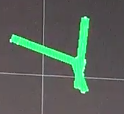
\includegraphics[width=0.4\linewidth]{images/ransac1.png}
  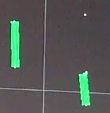
\includegraphics[width=0.4\linewidth]{images/ransac2.png}
  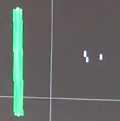
\includegraphics[width=0.4\linewidth]{images/ransac3.png}
  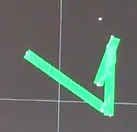
\includegraphics[width=0.4\linewidth]{images/ransac4.png}
  \caption{Lines extracted from the IR sensor data using the RANSAC method, from
  a single segment.}
  \label{fig:rsacseg}
\end{figure}

\subsubsection{Problems}
Examples of the lines extracted by the initial RANSAC process can be seen in
Figure~\ref{fig:rsacseg}. Examples of the result of the rotation and translation
process based on turn and odometry data can be seen in
Figure~\ref{fig:rsacline}.

There were numerous problems with the RANSAC approach. Firstly, there were some
issues with receiving odd sensor readings. This was mitigated by filtering the
sensor values with a minimum and maximum threshold. Some valid readings still
caused problems with the line extraction --- these points would not be removed,
and sometimes resulted in lines which were much longer than they should have
been, because the point was on the line model. There was also the problem of
RANSAC extracting lines with very few points remaining in the point cloud. This
issue was solved by adding a threshold on the minimum proportion of points in
the point cloud required for the algorithm to be run. Even with these additions,
some problems remained. Extraction would find diagonal lines, like in
Figure~\ref{fig:rsacseg}, and outliers would cause lines to be extended as
before. Sensor readings for maximum distance were being ignored, which meant
that regions of free space were not being properly defined when lines were used
to construct the map. Some of these problems could be mitigated by outlier
removal, splitting data into the left and right-hand data and running extraction
on those separately, and some post-processing on the extracted lines, such as
checking gradients. However, we were unable to implement any of these ideas
before the milestone deadline. Compounded with the issues with map construction,
the RANSAC method was abandoned and we moved on to trying to construct a simpler
topological map.

The map construction was also too simplistic. The bounding box of the lines is
not necessarily the correct region to define as empty space, especially since
there may be multiple different ``levels'' of walls in each segment. For
example, in segments where there are three parallel walls, one shorter than the
others, and in between them, then this wall will be entirely ignored, and the
space it occupies will be assumed to be free space.

The main reason for the unsuccessful implementation was a lack of good task
distribution and proper discussion about the approach. If we had discussed the
potential problems early on in the implementation, perhaps we would have not
chosen to take this approach and waste a lot of time.


\begin{figure}
  \centering
  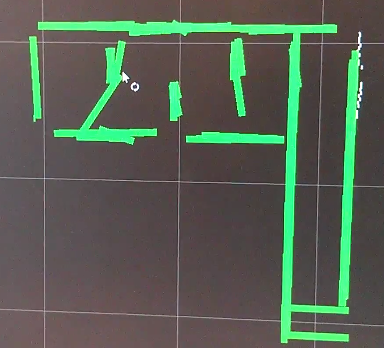
\includegraphics[width=\linewidth]{images/segmap.png}
  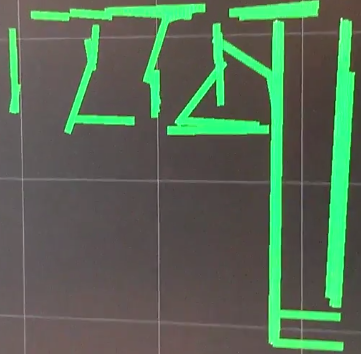
\includegraphics[width=\linewidth]{images/segmap2.png}
  \caption{Lines extracted from the IR sensor data using the RANSAC method,
    rotated and translated according to the turning information and odometry
    data. }
  \label{fig:rsacline}
\end{figure}

\subsection{Topological Map}
In place of the RANSAC based map, we decided to implement a basic topological
map which would place nodes at coordinates where the robot made a turn or
detected an object. Node coordinates were again based on the odometry. The
implementation saves the nodes to a bag file, which can then be read into the
system in the second phase. The map can then be used to navigate, and allows for
the addition of nodes into the existing map if new areas are explored.

We intended to add functionality to store information about potential areas for
exploration, and also to place nodes on the intersection points of lines to
improve the efficiency of navigation, but due to time restrictions we were
unable to complete these extensions.

\begin{figure}
  \centering
  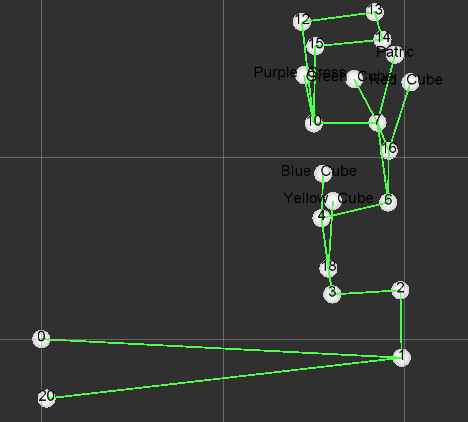
\includegraphics[width=0.4\linewidth]{images/map1.png}
  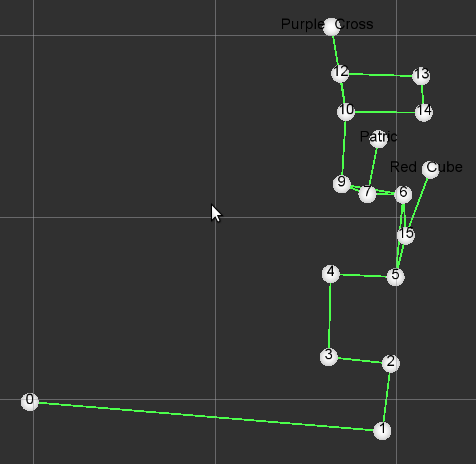
\includegraphics[width=0.4\linewidth]{images/map2.png}
  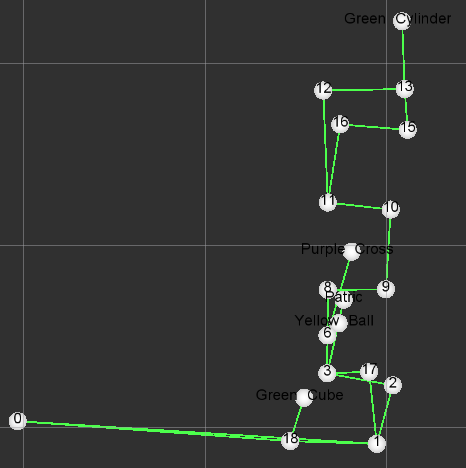
\includegraphics[width=0.4\linewidth]{images/map3.png}
  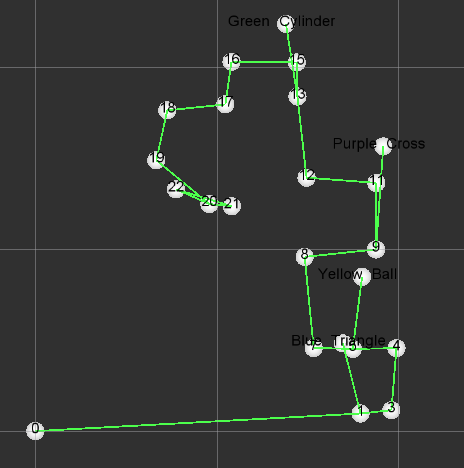
\includegraphics[width=0.4\linewidth]{images/map4.png}
  \caption{Examples of topological maps constructed from multiple runs in the
    same environment.}
  \label{fig:rsacline}
\end{figure}
\section{Odometry, Localisation and Navigation}
\subsection{Odometry}
The odometry was only facilitated through the use of motor encoders and careful controller tuning as to not let any slippage occur. Using the IMU was prematurely decided against since we had problems with the script that was running it. 
The odometry returned the total amount of distance travelled, the current heading and the absolute X and Y coordinates, all derived using the motion model of the robot, found \href{http://goo.gl/SGA99c}{here}.
\subsection{Localisation}
Localisation was implicit in Navigation as it did not include any filtering, i.e. localization was simply the task of referring the output of the odometry to the beginning of the coordinate system and thus to the node map, since it has metric data. That was done with a simple euclidean distance measure which was used as a threshold of whether the robot is on a certain node or not. 
\subsection{Navigation}
Navigation was implemented as a dual state system - either following the trajectory, described the map, or wallowing for when there were straight walls to help with the reduction of odometry error. While the wallfollowing was already well defined, we needed to implement the navigation capability separately. We used a BFS algorithm to find a path between two nodes. After that path following was done by using the difference of the vectors of the current position and that of the target (next accessible node of the path) and having this vector serve as the reference heading of the robot. Thus, there is a controller which makes sure the difference in angle between the heading of the robot and the reference vector is zero. That however added a serious problem - due to odometry errors the path was not always parallel to the walls, which meant that we needed to use a controller which aligns the map to the closest straight wall while the robot was following said map. This ensured that the map will always be aligned to the last seen wall, thereby reducing the error in heading significantly. Please note, that unfortunately we did not have time to implement an explorer which is capable of venturing away from the walls on its own accord, which meant that there was no point in investing time in tuning the tricky cascade of 3 controllers and the node got abandoned. 
Not all of it, though. A part of it got transplanted into the Advanced Explorer to create a new node under a new name - Fetch. This node uses localization to determine if the robot has reached the position from which a desired object can be seen. Of course it relays on the fact that the map is consecutive and deterministic, since we do not venture away from the walls very often. This meant that the task of fetching could be completed for about half of the objects. The Fetch node was proven to work in the lab, but was not used in the competition due to failure to get a map in the first run.   


\section{Work Environment}
\subsection{Version Control}
For source control, we used \texttt{git}, with repositories on GitHub. Each of
us had a separate account on GitHub, but we all committed to the same set of
repositories which were created in an Organisation on the site. We had separate
repositories for each major subsystem (mapping, controllers, vision, etc.).
Everyone committed to the same repositories, without using forks. While using
pull requests can have some benefits in terms of allowing team members to look
at what has been changed in a specific pull request and decide if changes are
required, in practice this sort of review process could only be done with a very
focused team that already have quite a lot of experience with \texttt{git}. It
would also be time consuming to have to do this, and time is already tight
enough as it is in the course. We tried to use a version of the branching model
described in \cite{nviebranch}. The idea is to use a branch \texttt{develop} in
each repository to develop code, branching off of that to develop new features,
in order not to force other members to pull code that is in the process of being
developed. The \texttt{master} branch is pushed to whenever a milestone
(release) is reached. While this may be a good branching model, in practice it
is perhaps not so useful if there is only one person working in a single
repository, as we often had. The good thing about it is that merging
\texttt{develop} into \texttt{master} only when a milestone is reached means
that the milestone code is easy to find, and it is possible to make sure that
only working code is merged.

There are some advantages to a multi-repository setup --- it is possible to work
on one repository completely independent of the others, which minimises the
number of merge commits and other issues that can be caused by having everything
in a single repository. The disadvantage of this is that all repositories have
to be pulled independently of each other, and if one forgets to do this it can
cause problems due to not having up to date code. The advantages of this setup
probably outweigh the disadvantages, however, because a single repository setup
would require more use of branches, which have issues of their own.

\subsection{System Setup}
At the beginning of the project we decided to make separate users on the NUC,
each with a separate \texttt{catkin} workspace. This worked well for us, as we
were able to work on different versions of code without affecting other members'
work. This came with the additional benefit that each member could launch their
own part of the code for a specific task independently. It did come with the
problem that each member had to pull updates to repositories, rather than having
a single repository which was up to date all the time. Each user belonged to the
same \texttt{robo} group, which allowed everyone to access each others' files. A
very useful script was one that allowed for execution of catkin make from any
directory, which saved having to switch between terminal windows or directories.
The system setup took some time, but the small amount of time spent at
the start was outweighed by the benefits.

\subsection{ROS Specifics}
We tried to keep to a specific structure for all nodes for consistency. Each
node created is an object (although there are no duplicated nodes). This keeps
the parameters of the node in its own scope, preventing possible issues with
clashes. Each node loads parameters and sets up subscribers in its constructor.
After all parameters are loaded, the node calls a function which executes the
main loop of the node. This structure makes it easy to see exactly what the node
is using by just looking at the constructor. In addition to this, we set up
parameter files for nodes which could use different parameter settings. Since
modifying extra parameters does not require recompilation, this saves time when
looking for the best parameter settings. A global parameter file was used to
store information about sensor positions and robot measurements. We make
extensive use of launch files as a result of this setup. Each launch file loads
the parameters that it requires. As such, it is possible to create a single
launch file at the top level which runs multiple nodes. Another parameter file
is used to define all topics that exist on the system. This means that one
change can change the name of the topic in all nodes which make use of it. This
means some additional parameter reading in nodes, but it lowers the likelihood
of bugs where nodes are not subscribing or publishing to the correct topics.

We implemented a utility library which was a wrapper around the parameter server
which would load a parameter into a given variable, depending on the type of the
variable. If the parameter was not present in the parameter server, an error
would be thrown with information about the missing parameter. This helped to
make parameter reading quicker and less prone to errors.

\section{Conclusion}

\nocite{*}
\printbibliography


\end{document}